\documentclass[10pt]{article}
\usepackage[margin=0.7in]{geometry}
\usepackage{graphicx,booktabs,amsmath,hyperref,mathptmx}
\hypersetup{colorlinks=true,urlcolor=blue}
\title{Direct signs expose the signed-cache tradeoff}
\author{Quadratic-twist study, PR2381}
\date{25 October 2026; direct-sign-20261025}
\begin{document}\sloppy\maketitle
\noindent\textbf{Executed comparison.} Native C++ and independent Rust execute
120 setups and 1,200 separate nonidentity main-source recoveries,40/400 per arm:
binary, direct uncached and setup-validated cached signs. All ten F43 size-two
policies/four roles remain; all 1,200 scalars verify. Both old arms match frozen
records. Every root, ordered lift, row/rank, full certificate, degree/witness,
promotion, base log, failed shift and scalar is equal. New hashes bind rejected
operand/sum tests too. A separate batch-RREF/witness audit checks 100 certificates.

\section*{A stronger reference changes the interpretation}
Direct uses P or one negation per operand without the binary scalar loop.
Cached setup still charges its entries, curve/sign checks and two inverse
validation additions. All signs in each query are tested even after a success.

\begin{center}\begin{tabular}{lrrr}\toprule
Prefix policy, separate $Q=P$; cold requests & Binary & Direct & Cached\\\midrule
Main point-add requests &125&45&47\\
Twist point-add requests &136&40&42\\
Main negations &20&20&2\\
Twist negations &24&24&2\\
Main scalar-loop iterations &54&14&14\\
Twist scalar-loop iterations &56&8&8\\
Main signed-operand reads &40&40&40\\
Twist signed-operand reads &48&48&48\\\bottomrule
\end{tabular}\end{center}
All 400 direct cold records use two fewer additions than cached. All 400 cached
records use fewer negations. Direct removes $4L$ additions and$2L$ scalar-loop
iterations relative to binary for $L$ tested signs, retaining its negations.
Cache replaces those negations by two at setup, at the cost of validation,
storage/reads. Neither arm dominates every request component.

\noindent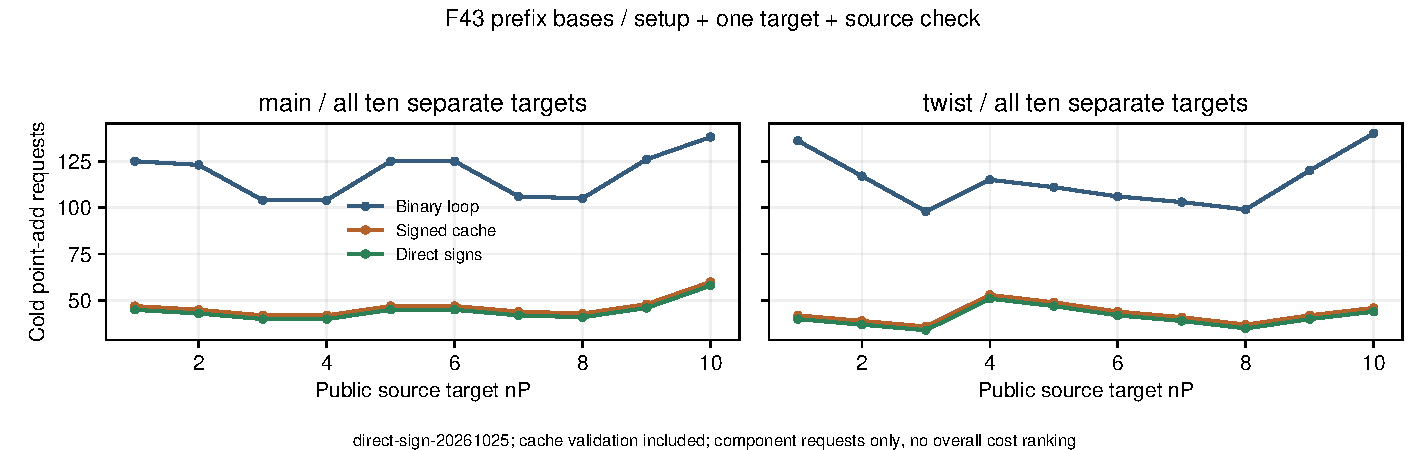
\includegraphics[width=\linewidth]{signs.pdf}

\noindent The old binary loop includes identity additions/unused doublings,
which compilers may optimize. These 38 differently weighted/nested requests are
not retired instructions or runtime. Cache checks/storage/reads, field tables,
hashing/trace work, allocation/sorting/traversal, exponentiation and audit remain
unpriced. No complete-work ranking, speedup, GAE, $S$, rho, intrinsic regularity
or fastest-external claim is admitted. The earlier component reduction is valid
against binary; it does not establish the value of caching against direct signs.

\newpage
\section*{Exact operands and existing proof bridge}
Every query binds the complete ordered tested tuples
$(i,j,s_i,s_j,A,B,A+B,\mathrm{accepted})$, including rejected signs.
Rust independently reconstructs these hashes, all 38 counters and the complete
mathematical outputs. Two new common counters, sign-operand reads and sign
dispatches, equal$2L$ in all arms. The older cache-only read counter is nested
and must not be counted again as equal-cost work. Hashes supply no solver answer.

Direct is the existing Lean \texttt{SignedCache.signedPoint} branch.
\texttt{signed\_eq\_zsmul}, \texttt{ordered\_lifts\_eq}, validated cache and
actual recovery theorems already prove the required group/list implications.
The actual cache, base logs and source annihilator are checked. No duplicate
theorem/new polynomial identity is introduced. The unmodified scoped gate
again passes 191 public/249 audited declarations, zero failing/extra trusted;
only propext, Classical.choice and Quot.sound. All 16 identity records remain;
\texttt{IDC1h202bb532af10c977} is rechecked with unchanged source/statement and
false identity/source controls. Native request execution is independently
replayed, not universally formalized.

\noindent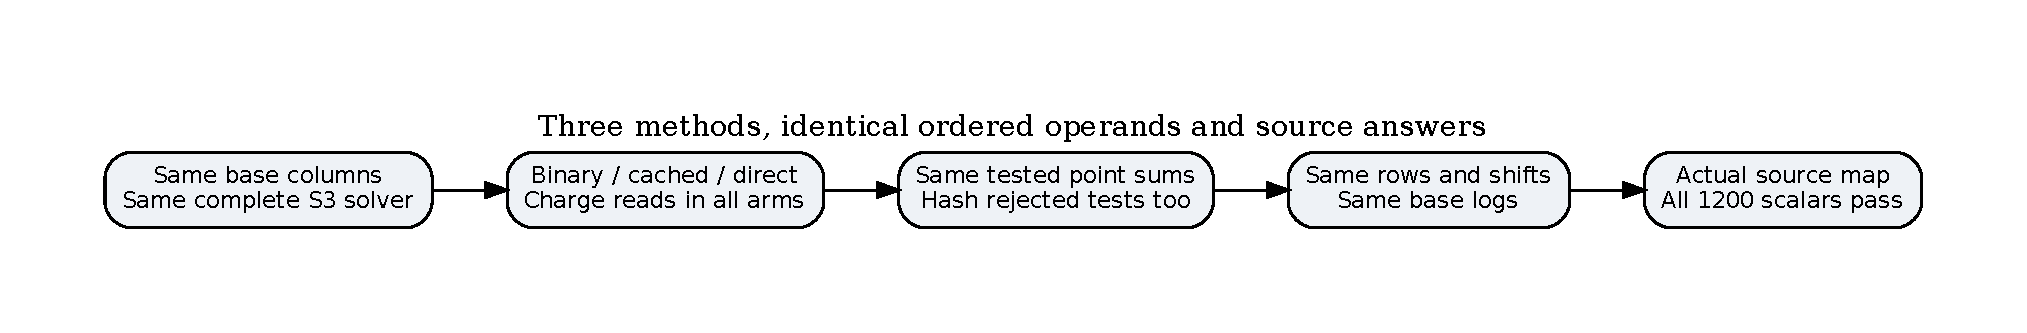
\includegraphics[width=\linewidth]{bridge.pdf}

\section*{Actual source DLP and all-policy results}
Main \texttt{icv1-fp6-t0-74779950} is$E:y^2=x^3+x$, $P=(31,18)$; twist
\texttt{icv1-fp6-t0-c6a8a47c} is$T:Y^2=X^3+4X$, $U=(24,26)$ over F43,
selected order11. The actual additive/injective map$(x,y)\mapsto(41x,11y)$
binds source recovery. This exceptional pair is base-field-isomorphic; U has
no EC1 registration. Recovery receives the point only, with labels outside it.

Summed hypothetical cold main/twist additions are 11750/11990 (binary),4398/4638
(cached),4198/4438 (direct). Negations are 1888/1888,200/200,1888/1888 respectively.
These sum 100 separate one-target records per role, not batch throughput or
independent curves. Direct/cached twist-addition lower/equal/higher counts
remain 43/1/56. Earlier first-query rank0/2, operational degree3/2 and equal
homogeneous cutoff2 remain. Both full setups reach coefficient rank2.

Seven rehashed controls reject without receipt: false direct trace/demand,
wrong on-curve cached sign point, missing arm/failed query, false scalar/source.
The fresh replay and 22 backend tests pass; full library and metadata checks are
recorded in validation. Profile remains unavailable through missing gawk,
Conductor exits127, and no paid resource/upload occurred.

\section*{Next actual transfer/yield lead}
The next proposed route uses already registered F13 models
\texttt{icv1-fp4-t0-6bee67e0} (a1,b4),
\texttt{icv1-fp4-t0-bb514d71} (a4,b7) and
\texttt{icv1-fp4-t0-097da6b6} (a4,b6). A standard degree-two coordinate
candidate, including the final scaling to the d2 monic twist, is
\[
 x'=12(x+2/(x-10)),\qquad y'=8y(1-2/(x-10)^2).
\]
\noindent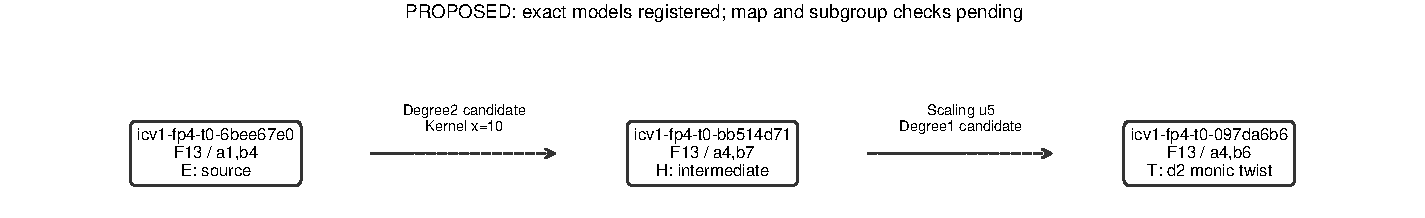
\includegraphics[width=\linewidth]{route.pdf}
This is a proposed construction, not an executed reduction here. Check
infinity/kernel/poles, actual equations, r7 scalar transport/injectivity and
non-isomorphism before comparing all size-two bases and useful S3 rows/degrees.
Matched-base conservation and all losses remain. No registry/catalog change
or upload is needed for these existing models. The cubic j0 option is deferred,
not refuted. General geometry, stationary yield, calibrated cost, shared
coordination, review and CI/integration remain open.
Full sources, proof links, commands and receipts are in the accompanying README.
\end{document}
